\documentclass[a4paper]{article}
\usepackage[utf8]{inputenc}
\usepackage[russian,english]{babel}
\usepackage[T2A]{fontenc}
\usepackage[left=10mm, top=20mm, right=18mm, bottom=15mm, footskip=10mm]{geometry}
\usepackage{indentfirst}
\usepackage{amsmath,amssymb}
\usepackage{mathastext} 
\usepackage[italicdiff]{physics}
\usepackage{graphicx}
\usepackage{caption}
\usepackage{float}
\usepackage{caption}
\renewcommand{\thefootnote}{\fnsymbol{footnote}}
\usepackage{tablefootnote}
\usepackage{footmisc}
\usepackage{textcomp}
\usepackage{multicol}
\usepackage{multirow}
\usepackage[parfill]{parskip}
\usepackage{makecell}
\usepackage{array}  
\usepackage{siunitx}
\usepackage{booktabs}
\sisetup{
    exponent-product = \cdot,
    per-mode = symbol,
    separate-uncertainty = true,
    uncertainty-separator = \,
}
\renewcommand\cellalign{cc} 
\renewcommand\cellgape{\Gape[2pt]} 
\usepackage[utf8]{inputenc}\newcommand{\approxtext}[1]{\ensuremath{\stackrel{\text{#1}}{\approx}}}
\usepackage[colorlinks=true, urlcolor=blue, linkcolor=blue, citecolor=blue]{hyperref}
\graphicspath{{images/}}
\DeclareGraphicsExtensions{.pdf,.png,.jpg}
\usepackage{wrapfig}
\captionsetup{labelformat=empty}
\usepackage{caption}
\captionsetup[figure]{name=Рисунок}
\captionsetup[table]{name=Таблица}
%\usepackage{newtxtext,newtxmath} 
\title{\textbf{Отчет о выполнении лабораторной работы 4.4.1}}
\date{}
\author{Котляров Михаил, Б01-402}

\begin{document}

\maketitle
	
\section{Введение}

\subsubsection*{Цель работы:} Знакомство с работой и настройкой гониометра Г5, определение спектральных характеристик амплитудной решётки.

\subsubsection*{Оборудование и инструментальные погрешности}

\textbf{гониометр Г-5}: погрешность измерения $\sigma_\varphi = 5''$,\\
\textbf{дифракционная решётка}: Период $500 \, \frac{\text{штрих}}{\text{мм}} $ ($d = 2$ мкм),\\
\textbf{ртутная лампа}.

\subsection*{Теоретические сведения}

Основное соотношение приближенной теории дифракционной решётки:

	\begin{equation}
	d\sin \varphi_m = m\lambda.
 \label{main}
	\end{equation}
 
Угловая дисперсия $D$ характеризует угловое расстояние между близкими спектральными линиями:
	\begin{equation}
	D = \frac{d\varphi}{d\lambda} = \frac{m}{d \cos \varphi}=\frac{m}{\sqrt{d^{2}-m^{2} \lambda^{2}}}.
	\label{Dispersion}
	\end{equation}

Рассмотрим изображения спектра для двух узких спектральных линий с длинами волн $\lambda$ и $\lambda+\delta\lambda$. Для минимального значения $\lambda+\delta\lambda$, которое может быть определено по результатам измерений, вводят важнейшую характеристику спектрального прибора — разрешающую способность:

\begin{equation}
    R=\frac{\lambda}{\delta\lambda} = \frac{\varphi}{\delta \varphi}.
\end{equation}

\subsection*{Схема установки}
\subsubsection*{Устройство гониометра}

Оптическая схема гониометра представлена на рис. 1а. Свет от источника $S$ проходит через коллиматор (устройство, дающее параллельный пучок, состоящее из щели 1 и объектива 5 ) и преобразуется призмой или решёткой в набор параллельных пучков, каждый из которых соответствует определённой длине волны.

A)
\begin{center}
    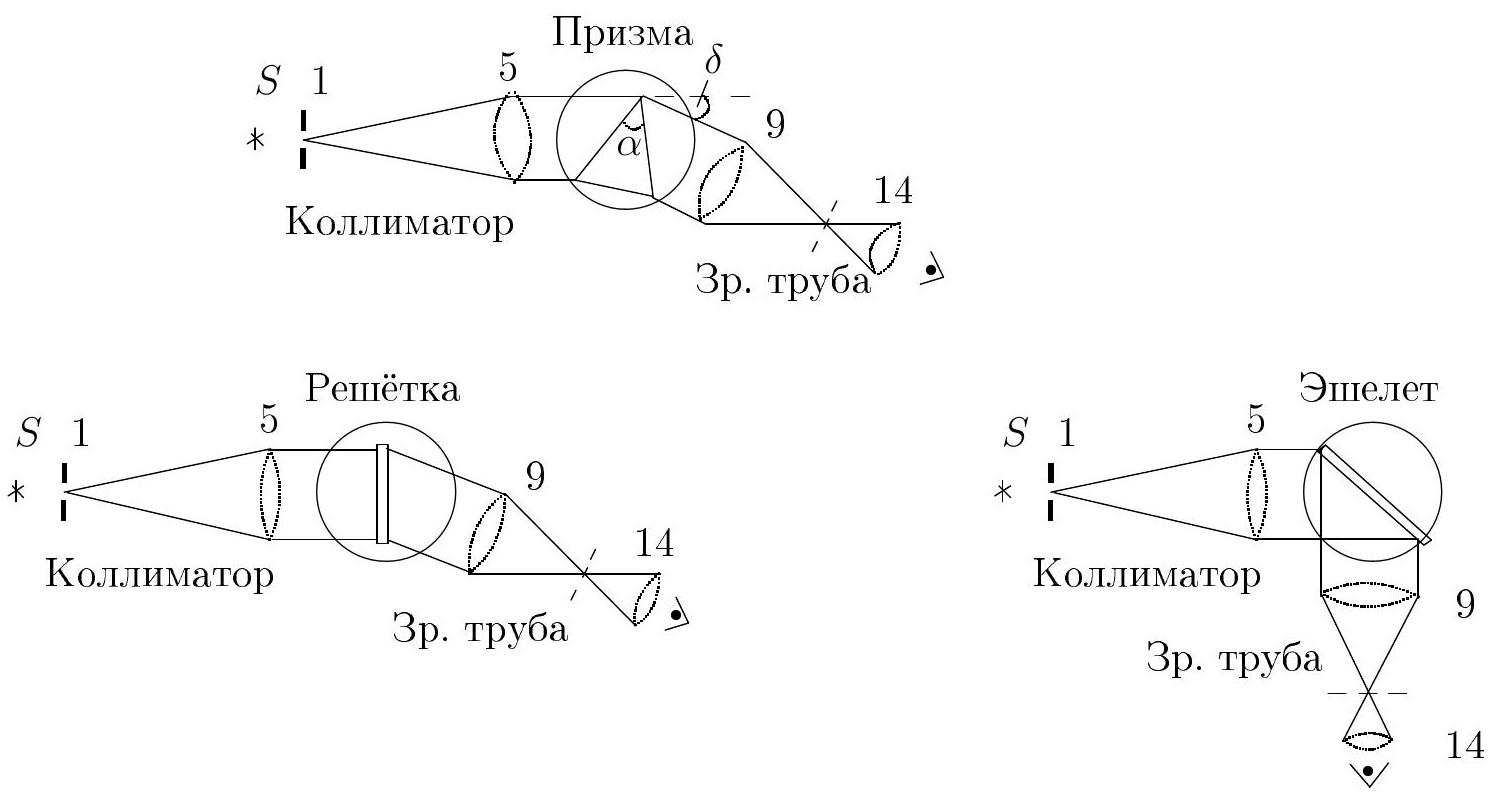
\includegraphics[scale=0.2]{Pictures/2023_04_02_a48ae02e429ba186bcd7g-2}
\end{center}


Б)

\begin{center}
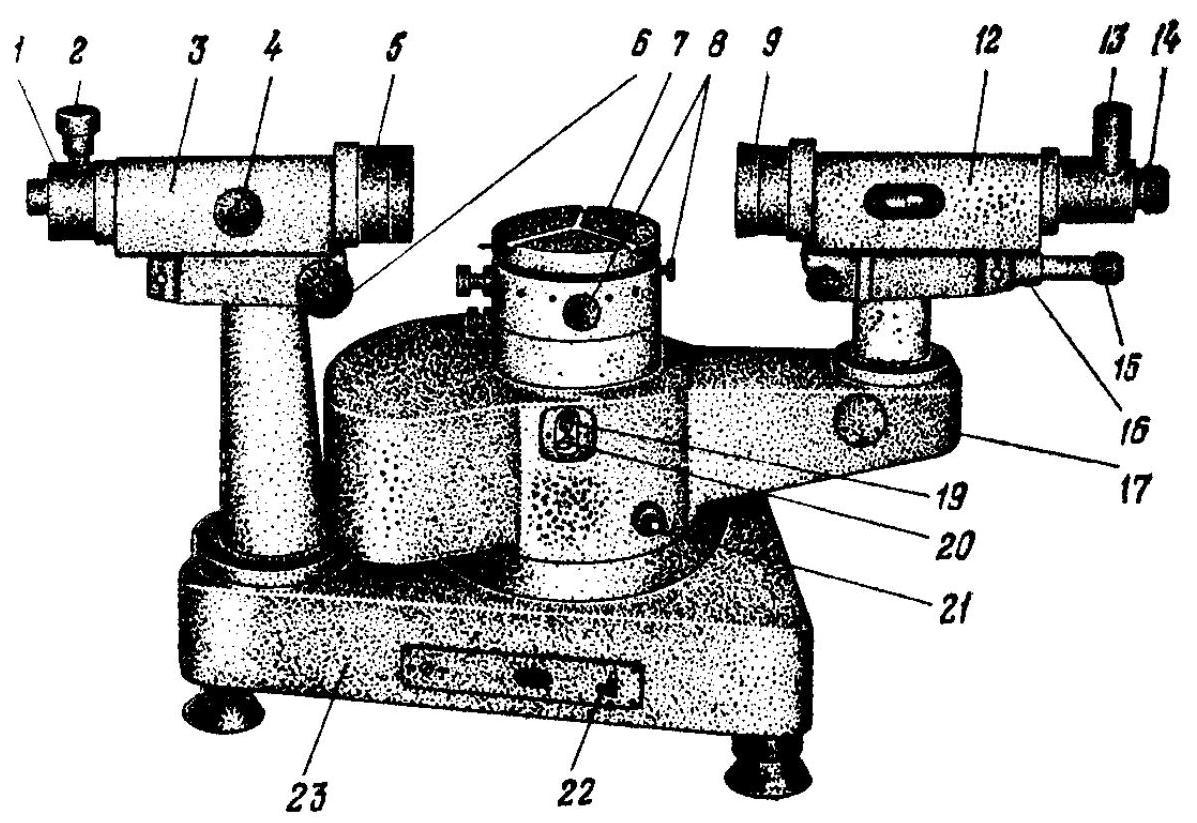
\includegraphics[scale=0.2]{Pictures/2023_04_02_a48ae02e429ba186bcd7g-2(2)}
\end{center}

B)

\begin{center}
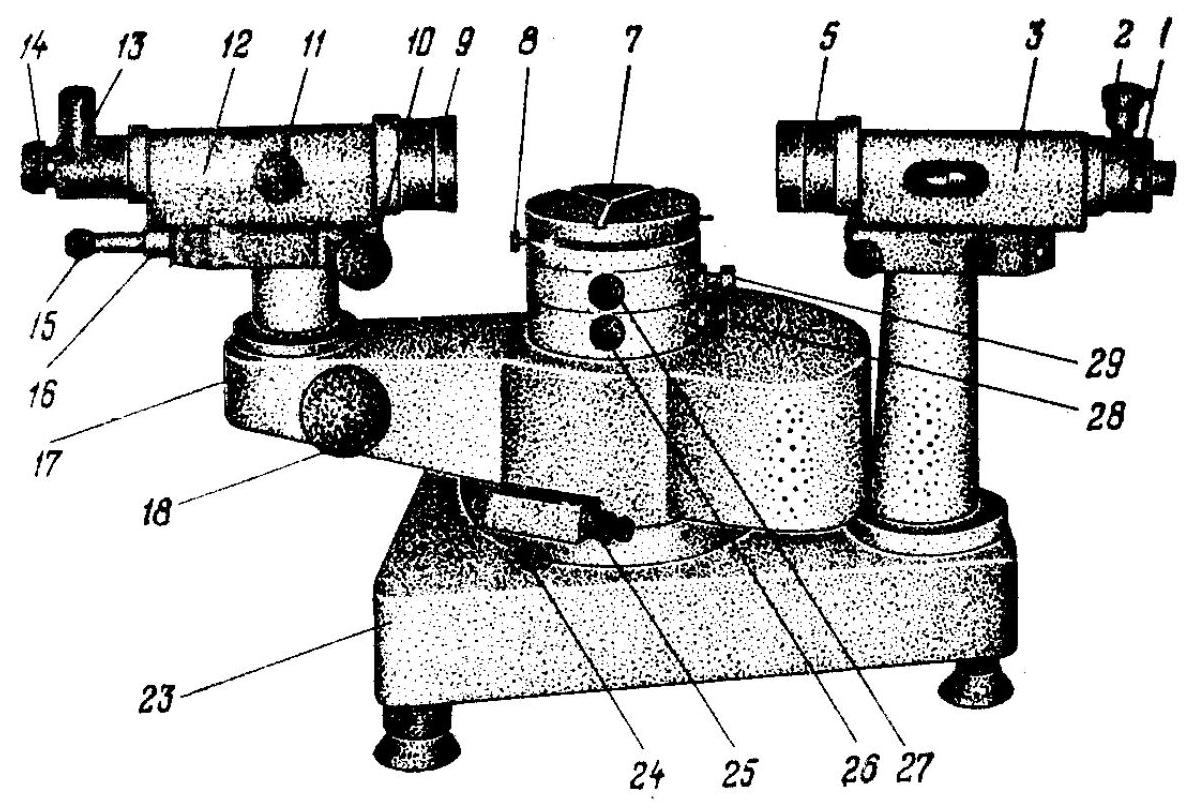
\includegraphics[scale=0.2]{Pictures/2023_04_02_a48ae02e429ba186bcd7g-2(1)}

Рис. 1. Оптическая схема и внешний вид гониометра

\end{center}


Параллельные пучки собираются в фокальной плоскости объектива 9 зрительной трубы и рассматриваются глазом через окуляр 14. При освещении щели ртутной лампой, дающей дискретный спектр, в фокальной плоскости видны отдельные линии - цветные изображения входной щели.

Внешний вид гониометра представлен на рис. 1. Коллиматор 3, столик 7 и алидада 17 со зрительной трубой 12 крепятся на массивном основании 23. На столике 7 размещаются исследуемые объекты. Коллиматор закреплён неподвижно, а столик и алидада с трубой могут вращаться вокруг вертикальной оси.

Ширину коллиматорной щели можно менять от 0 до 2-х мм при помощи микрометрического винта 2 , высоту - от 0 до 2-х см - при помощи диафрагмы с треугольным вырезом («ласточкин хвост»), надетой на щель. Винт 4 служит для перемещения объектива 5 - настройки коллиматора на параллельный пучок.

Зрительная труба 12 состоит из объектива 9 и окуляра 14 с автоколлимационным устройством 13. Объективы коллиматора и зрительной трубы одинаковы. Фокусировка трубы производится винтом 11. Наклон коллиматора и зрительной трубы к горизонтальной оси изменяется винтами 6 и 10 соответственно.

Схема окуляра О зрительной трубы с автоколлимационным устройством приведена на рис. 2а. Свет от лампы Л проходит через защитную стеклянную пластинку П и попадает на автоколлимационную сетку А, содержащую две взаимно перпендикулярные щели. Свет, прошедший через сетку А (светящийся крест - рис. 2б), попадает на две прямоугольные призмы $P$ и отражается от гипотенузной грани, на которую нанесён полупрозрачный слой с коэффициентом отражения $50 \%$.

а)
\begin{figure}[H]
    \centering
    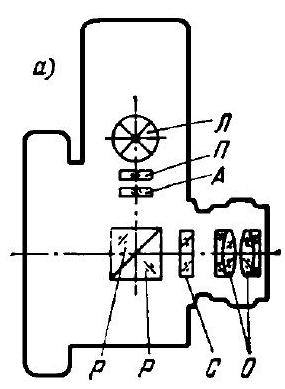
\includegraphics[scale=0.4]{Pictures/2023_04_02_a48ae02e429ba186bcd7g-1(1)}

б)
    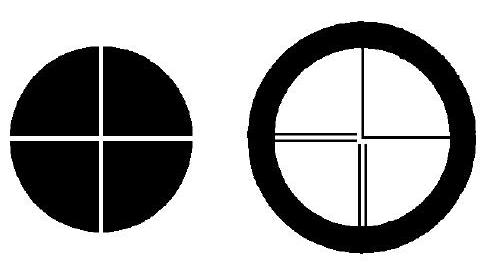
\includegraphics[scale=0.4]{Pictures/2023_04_02_a48ae02e429ba186bcd7g-1}\\
    {Рис. 2: Автоколлимационное устройство}
    \label{fig:my_label}
\end{figure}


Для юстировки гониометра на столик ставится предмет с плоской отражающей поверхностью. После отражения от неё параллельный пучок лучей возвращается назад в зрительную трубу и собирается в фокальной плоскости объектива. В этом случае светящийся автоколлимационный крест можно увидеть через окуляр зрительной трубы. Кроме того, в окуляре имеется ещё одна сетка C, на которой изображён чёрный отсчётный крест. Совмещённые изображения обоих крестов рассматриваются через окулярные линзы О. Резкость видимого изображения отсчётного креста регулируется вращением оправы окуляра трубы.

Обе сетки окуляра, А и C (рис. 2а), расположены на строго одинаковых расстояниях от гипотенузных граней призмы $P$, поэтому их одновременное наблюдение в окуляре возможно только при совпадении фокальных плоскостей объектива и окуляра (труба настроена на бесконечность).

Важнейшим узлом гониометра является устройство, служащее для отсчёта угла поворота зрительной трубы вокруг вертикальной оси, проходящей через центр столика. На этой оси крепится прозрачное кольцо (лимб), расположенное в корпусе прибора. На поверхности лимба нанесена шкала с делениями. Лимб разделён на $3 \times 360=1080$ делений. Цена деления $20^{\prime}$, оцифровка делений произведена через $1^{\circ}$. Шкалу лимба можно наблюдать через окуляр отсчётного устройства 16 при включённой подсветке (тумблер 22). Резкость изображения шкалы регулируется вращением оправы окуляра 15.

Оптическая система отсчётного устройства собрана так, что через окуляр можно наблюдать изображения штрихов двух диаметрально противоположных участков лимба, причём одно изображение прямое, а другое обратное. Кроме того, оптическая система позволяет перемещать эти изображения друг относительно друга, оставляя в покое как лимб, так и алидаду со зрительной трубой. Это перемещение штрихов измеряется при помощи оптического микрометра. Шкала микрометра рассчитана таким образом, что при перемещении её на 600 делений верхнее изображение штрихов лимба смещается относительно нижнего на 10'. Следовательно, цена деления шкалы микрометра $1^{\prime \prime}$.

Для удобства экспериментатора в гониометре предусмотрено несколько вариантов относительного вращения столика, алидады со зрительной трубой и лимба.
Отсчётное устройство гониометра обеспечивает точность измерения угла не хуже $5^{\prime \prime}$.

\section{Ход работы и обработка результатов}

\section{Выполнение и обработка результатов}

\subsection{Определение периода дифракционной решётки}

С помощью гониометра измерим углы дифракции для основных линий спектра ртути в порядке  $m = +1$ и \\ $m = -1$. Измерения будем проводить при симметричном ходе лучей, когда плоскость решётки перпендикулярна оси коллиматора. Нулевой порядок ($m = 0$) соответствует углу $\varphi_0 = 180^\circ$, относительно которого будем отсчитывать углы дифракции. Полученные значения углов $\varphi_{+1}$ и $\varphi_{-1}$ для каждой спектральной линии занесём в таблицу.


Для каждого угла вычислим синус, а также его абсолютную погрешность, обусловленную погрешностью измерения угла $\Delta\varphi = 5''$. Погрешность синуса найдём по формуле
\[
\Delta(\sin\varphi) = |\cos\varphi|\,\Delta\varphi_\text{рад},
\]
где $\Delta\varphi_\text{рад}$ – погрешность угла в радианах.

% Таблица 1
\begin{table}[h!]
    \centering
    \begin{tabular}{|c|c|c|c|c|c|c|c|}
        \hline
        цвет & $\lambda$, нм & $\varphi_{+1}$ & $\sin\varphi_{+1} \pm \Delta\sin\varphi_{+1}$ & $\varepsilon_{\sin\varphi_{+1}}$, \% & $\varphi_{-1}$ & $\sin\varphi_{-1} \pm \Delta\sin\varphi_{-1}$ & $\varepsilon_{\sin\varphi_{-1}}$, \% \\ \hline
        фиолетовый & 404,7 & $167^\circ 19' 4''$ & $0{,}21954 \pm 0{,}00002$ & 1,08 & $192^\circ 32' 39''$ & $-0{,}21719 \pm 0{,}00002$ & 1,09 \\ \hline
        синий & 435,8 & $165^\circ 39' 2{,}5''$ & $0{,}24783 \pm 0{,}00002$ & 0,95 & $193^\circ 59' 59''$ & $-0{,}24192 \pm 0{,}00002$ & 0,97 \\ \hline
        голубой & 491,6 & $165^\circ 31' 0''$ & $0{,}25010 \pm 0{,}00002$ & 0,94 & $194^\circ 7' 31''$ & $-0{,}24404 \pm 0{,}00002$ & 0,96 \\ \hline
        зеленый & 546,1 & $164^\circ 00' 21''$ & $0{,}27554 \pm 0{,}00002$ & 0,85 & $195^\circ 45' 23{,}5''$ & $-0{,}27155 \pm 0{,}00002$ & 0,86 \\ \hline
        Желтый 1 & 577 & $163^\circ 3' 57''$ & $0{,}29127 \pm 0{,}00002$ & 0,80 & $196^\circ 39' 41''$ & $-0{,}27564 \pm 0{,}00002$ & 0,85 \\ \hline
        Желтый 2 & 579,1 & $162^\circ 59' 38''$ & $0{,}29247 \pm 0{,}00002$ & 0,79 & $196^\circ 43' 44''$ & $-0{,}28784 \pm 0{,}00002$ & 0,81 \\ \hline
    \end{tabular}
    \caption{Таблица 1. Значения углов и синусов для порядков $+1$ и $-1$}
    \label{tab:sin_phi}
\end{table}

Построим график зависимости $\sin\varphi$ от длины волны $\lambda$ для порядков $+1$ и $-1$ (рис.~\ref{fig:sin}). Согласно формуле дифракционной решётки
\[
d\sin\varphi = m\lambda,
\]
при $m = \pm 1$ зависимость $\sin\varphi(\lambda)$ является линейной с угловым коэффициентом $k = \pm 1/d$. Аппроксимируем экспериментальные точки прямой $y = a\lambda + b$ методом наименьших квадратов с учётом погрешностей $\Delta(\sin\varphi)$.

\begin{figure}[h!]
\centering
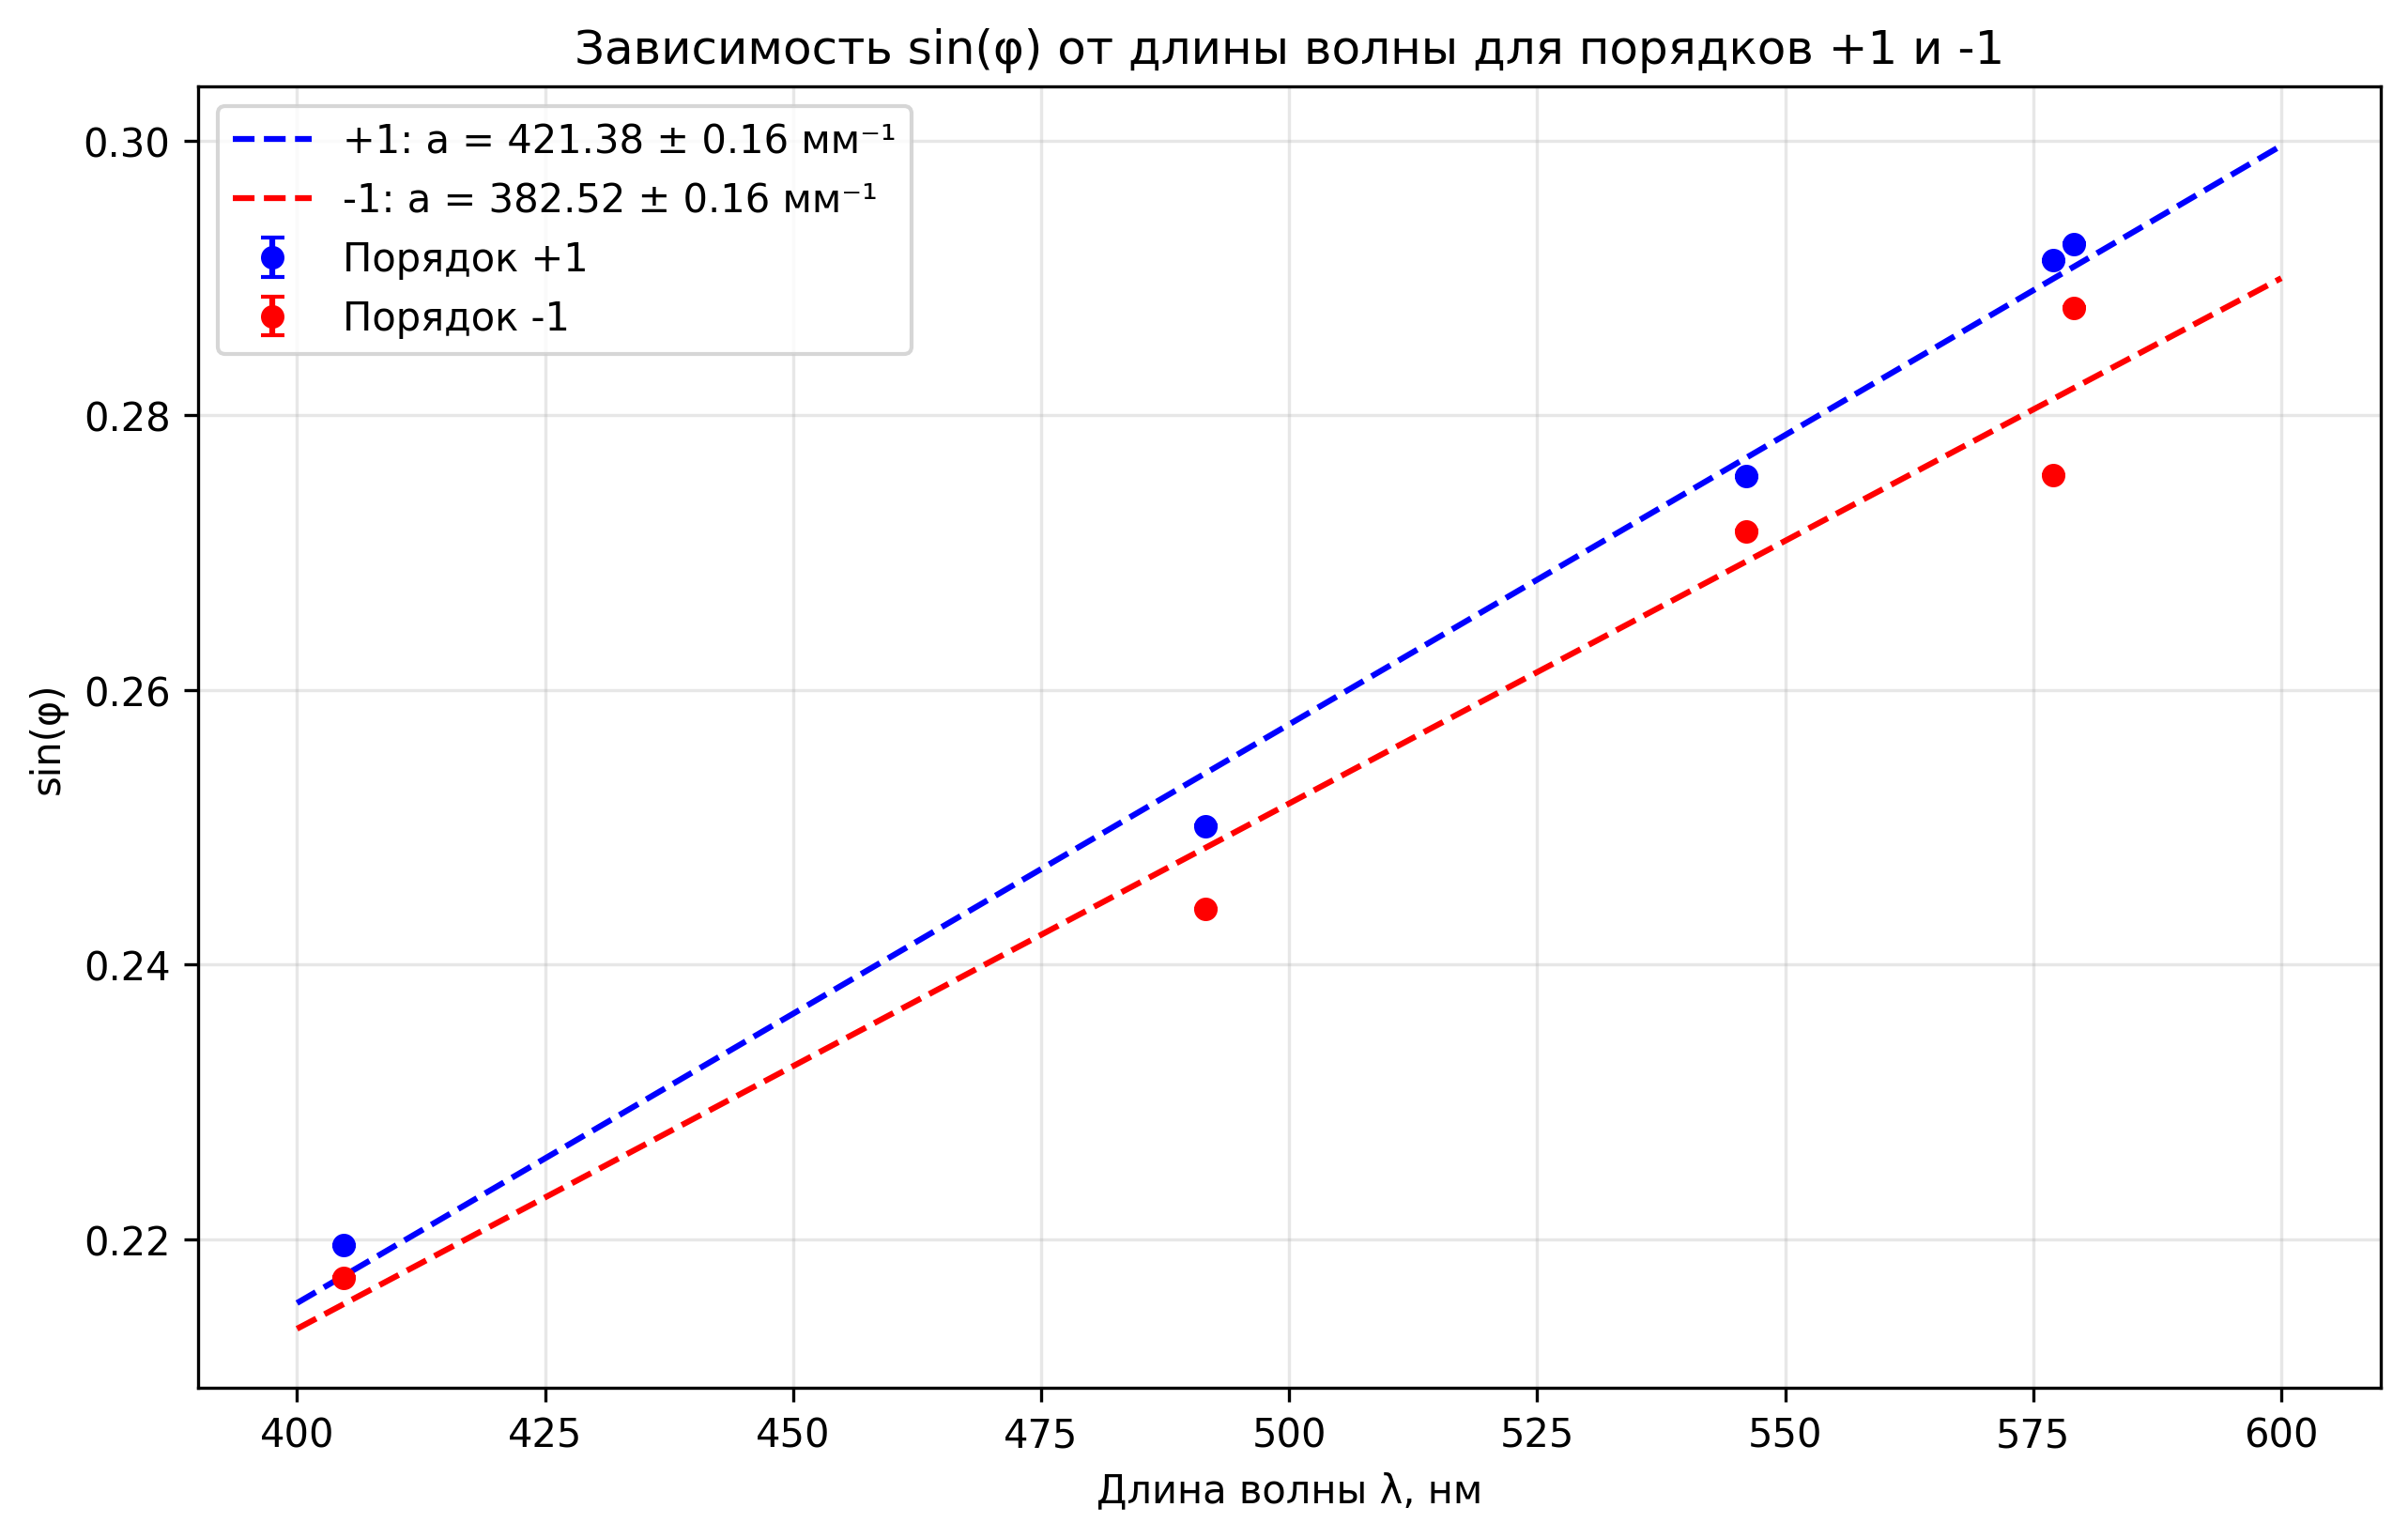
\includegraphics[width=0.7\textwidth]{Graphics/sin_vs_lambda_fit.png}
\caption{График 1. Зависимость $\sin\varphi$ от длины волны для порядков $+1$ и $-1$}
\label{fig:sin}
\end{figure}

Точки с длиной волны  435,8 (синий цвет) не учитывались, поскольку в эксперименте они были видны плохо и не ложатся на прямую. Так же для порядка $m = -1$ значение синуса инвертировано для сравнения с $m = 1$.\\
В результате аппроксимации получили следующие значения коэффициентов: $a_{+1} = 421,38 \pm 0,16 \,\frac{\text{штрих}}{\text{мм}}$, \\$a_{-1} = 382,52 \pm 0,16 \,\frac{\text{штрих}}{\text{мм}}$. Угловой коэффициент равен $1/d$, следовательно, период решётки
\[
d = \frac{1}{a}.
\]
Подставляя численные значения, нашли
\[
d_{+1} =  2,373 \pm 0,001 \, \text{мкм}.
\]
Аналогично из данных для порядка $-1$ получили $d_{-1} = 2,614 \pm 0,001$ мкм. Усреднённое значение периода составляет
\[
d_\text{ср} = 2,494\pm 0,001\ \text{мкм} \, (\varepsilon_{d_\text{ср}} = 0,03 \%).
\]
Паспортное значение решётки – 500 штрихов на миллиметр, что соответствует периоду $d_\text{пасп} = 2,000$ мкм.

\subsection{Угловая дисперсия}

Для исследования угловой дисперсии измерим угловые координаты обеих линий жёлтого дублета ($\lambda_1 = 577,0$ нм, $\lambda_2 = 579,1$ нм) в порядках $m = \pm1,\ \pm2$. Полученные углы занесём в таблицу.

Разность длин волн жёлтого дублета составляет $\Delta\lambda = 2,1$ нм = 21 Å. Угловое расстояние между линиями $\Delta\varphi = |\varphi_{579} - \varphi_{577}|$ переведём в угловые секунды. Экспериментальную угловую дисперсию вычислим как
\[
D_\text{эксп} = \frac{\Delta\varphi}{\Delta\lambda}.
\]

Теоретическая угловая дисперсия для дифракционной решётки определяется формулой
\[
D_\text{теор} = \frac{m}{d\cos\varphi} = \frac{m}{\sqrt{d^2-m^2\lambda^2}},
\]
где $\varphi$ – угол дифракции для средней длины волны $\lambda_\text{ср} = 578,05$ нм. Используя найденное значение периода $d = 2,000$ мкм, для каждого порядка рассчитаем теоретические значения дисперсии.


\begin{table}[h!]
    \centering
    \begin{tabular}{|c|c|c|c|}
        \hline
        порядок & 1-ая линия & 2-ая линия \\ \hline
        1 & $163^\circ 3'57''$ & $162^\circ 59'38''$ \\ \hline
        -1 & $196^\circ 39'41''$ & $196^\circ 43'44''$ \\ \hline
        2 & $143^\circ 51'38''$ & $143^\circ 42'12''$ \\ \hline
        -2 & $214^\circ 33'11''$ & $214^\circ 42'19''$ \\ \hline
    \end{tabular}
    \caption{Таблица 2. Углы для жёлтого дублета}
    \label{tab:yellow_angles}
\end{table}

На графике ~\ref{fig:disp} представлена зависимость угловой дисперсии от порядка спектра. Точками показаны экспериментальные значения с крестами погрешностей, сплошной линией – теоретическая кривая, рассчитанная по формуле для непрерывного изменения $m$.

\begin{figure}[h!]
\centering
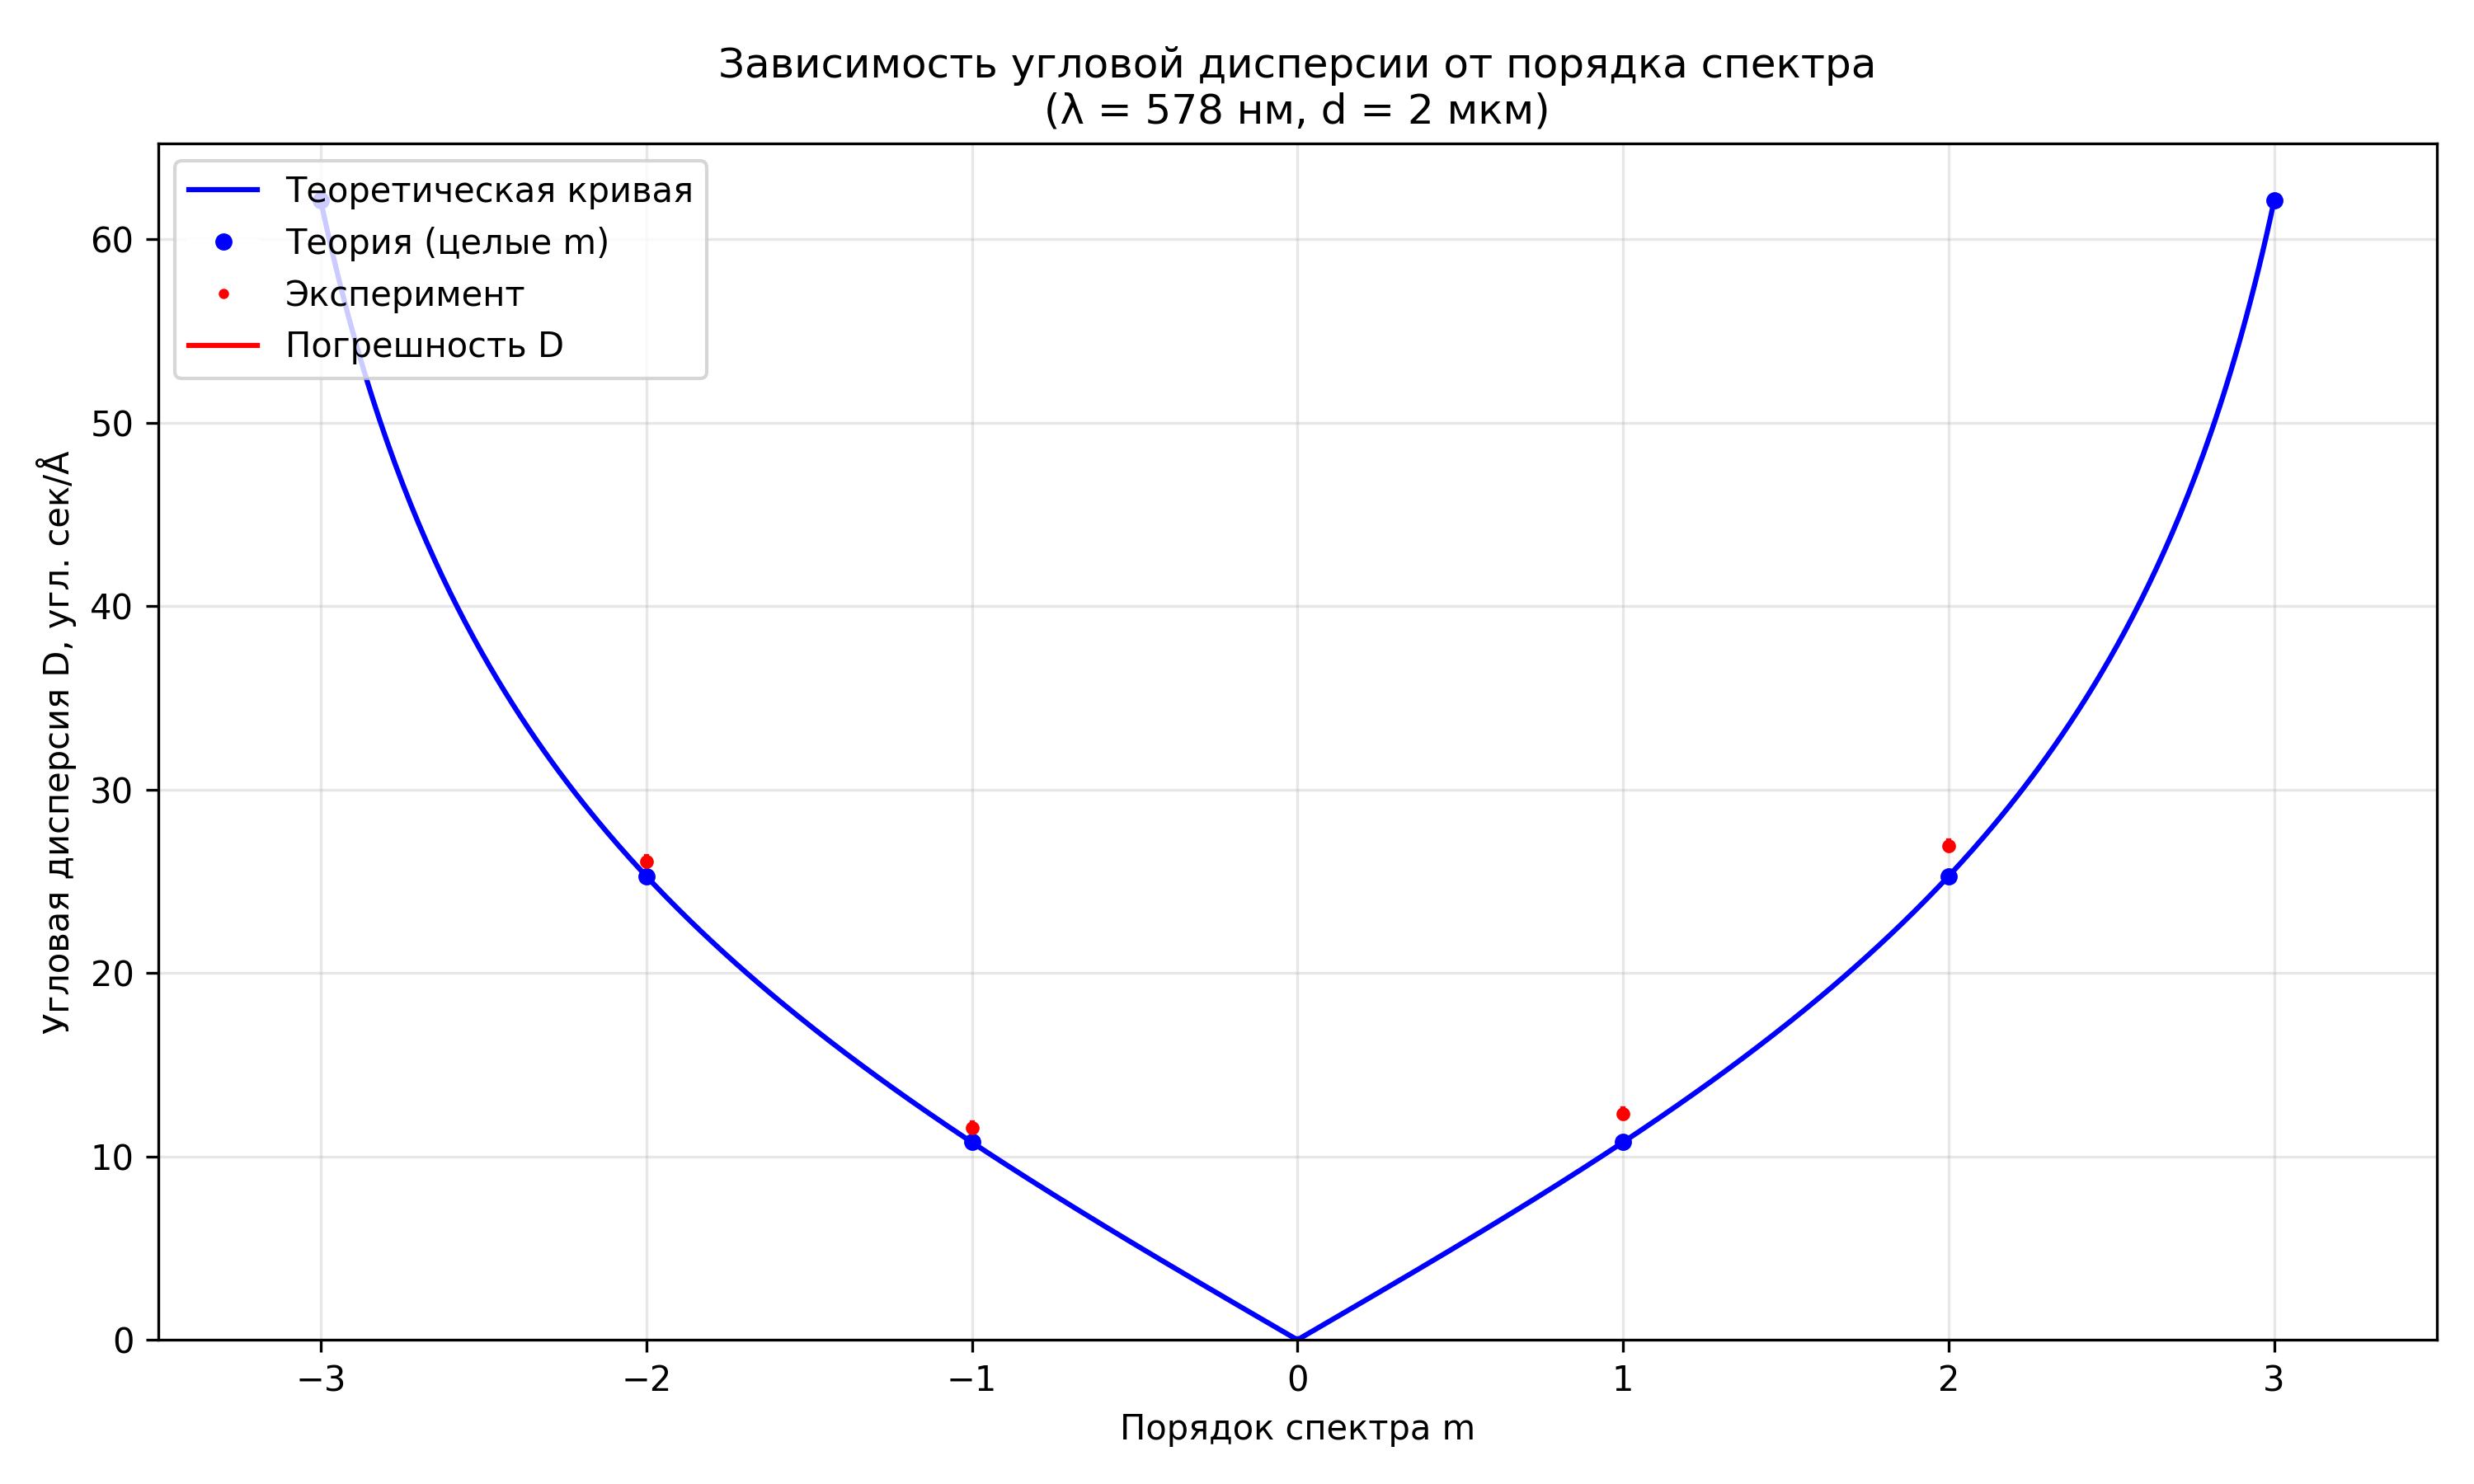
\includegraphics[width=0.7\textwidth]{Graphics/dispersion_vs_m.png}
\caption{График 2. Зависимость угловой дисперсии от порядка спектра}
\label{fig:disp}
\end{figure}

Сравнение экспериментальных и теоретических значений приведено в таблице.

\begin{table}[h!]
    \centering
    \begin{tabular}{|c|c|c|c|c|c|}
        \hline
        № & $D_{\text{эксп}} \pm \Delta D_{\text{эксп}}, \, \frac{\text{уг.сек}}{\text{Å}}$  & $\varepsilon_{\text{эксп}}$, \% & $D_{\text{теор}}, \, \frac{\text{уг.сек}}{\text{Å}}$ & $|\Delta D|, \, \frac{\text{уг.сек}}{\text{Å}}$ & $\delta$, \% \\ \hline
        1 & $12{,}333 \pm 0{,}238$ & 1,93 & $10{,}773$ & 1,560 & 14,48 \\ \hline
        2 & $11{,}571 \pm 0{,}238$ & 2,06 & $10{,}773$ & 0,798 & 7,41 \\ \hline
        3 & $26{,}952 \pm 0{,}238$ & 0,88 & $25{,}278$ & 1,674 & 6,62 \\ \hline
        4 & $26{,}095 \pm 0{,}238$ & 0,91 & $25{,}278$ & 0,817 & 3,23 \\ \hline
    \end{tabular}
    \caption{Таблица 3. Сравнение экспериментальной и теоретической угловой дисперсии для жёлтого дублета ртути}
    \label{tab:dispersion_hg}
\end{table}

Получили, что наблюдается хорошее согласие экспериментальных данных с теорией в пределах погрешностей измерений. Небольшие систематические расхождения могут быть связаны с неточностью юстировки или погрешностью определения периода решётки.

\subsection{Разрешающая способность}

Для оценки разрешающей способности измерим угловую ширину одной из линий жёлтого дублета ($\lambda = 577$ нм) в порядке $m = +1$. Измерения будем проводить при минимальной ширине входной щели, когда дальнейшее её уменьшение не приводит к сужению линии. Расстояние между первыми нулями интенсивности примем за полную ширину $2\delta\varphi$; полуширина $\delta\varphi = 152''$ равна половине этого расстояния.

Минимально разрешимый интервал длин волн $\delta\lambda$ найдём из соотношения
\[
\delta\lambda = \frac{\delta\varphi}{D_\text{эксп}},
\]
где $D_\text{эксп}$ – угловая дисперсия для данного порядка (в радианах на нанометр). Вычислим экспериментальную разрешающую способность
\[
R_\text{эксп} = \frac{\lambda}{\delta\lambda} = D_\text{эксп} \frac{\lambda}{\delta\varphi} = 409 \pm 13 \, (\varepsilon_{R_\text{эксп}} = 3,29 \%).
\]

Теоретическая разрешающая способность дифракционной решётки определяется выражением
\[
R_\text{теор} = mN,
\]
где $N$ – полное число освещённых штрихов. $N = 409$ штрихов.
Размер освещенной части $l = N * d \approx 817,9$ мкм.

\subsection{Дисперсионная область}

Определим порядок спектра, при котором происходит наложение фиолетовой линии ($\lambda_\text{ф} = 435,8$ нм) на жёлтую ($\lambda_\text{ж} = 579,1$ нм). Условие перекрытия спектров соседних порядков:
\[
m\lambda_\text{ж} = (m+1)\lambda_\text{ф}.
\]
Отсюда
\[
m = \frac{\lambda_\text{ф}}{\lambda_\text{ж} - \lambda_\text{ф}} = \frac{435,8}{579,1 - 435,8} \approx \frac{435,8}{143,3} \approx 3,04.
\]
Таким образом, наложение ожидается уже при $m = 3$. Визуально в нашей установке спектры до $m = 2$ не перекрываются, что согласуется с расчётом.

Дисперсионная область для порядка $m$ может быть найдена по формуле
\[
\Delta\lambda = \frac{\lambda}{m}.
\]
Для $\lambda = 578$ нм и $m = 2$ получили $\Delta\lambda \approx 289$ нм, что значительно превышает ширину исследуемого участка спектра.

\section{Результаты и обсуждения}

В ходе выполнения работы были проведены измерения углов дифракции для основных линий спектра ртути в порядках $m = \pm1$ (табл.~\ref{tab:sin_phi}) и для жёлтого дублета в порядках $m = \pm1,\ \pm2$ (табл.~\ref{tab:yellow_angles}). На основе этих данных определены основные характеристики дифракционной решётки и проверены теоретические зависимости.

\subsection{Период решётки}
Из графика зависимости $\sin\varphi$ от длины волны (рис.~\ref{fig:sin}) методом наименьших квадратов получены значения периода:
\[
d_{+1} = 2{,}373 \pm 0{,}001\ \text{мкм},\quad d_{-1} = 2{,}614 \pm 0{,}001\ \text{мкм}.
\]
Среднее значение составило $d_\text{ср} = 2{,}494 \pm 0{,}001\ \text{мкм}$ (относительная погрешность $0{,}03\%$). Паспортное значение решётки ($500$ штрихов/мм) соответствует $d_\text{пасп} = 2{,}000\ \text{мкм}$. Наблюдаемое расхождение ($\approx 25\%$) значительно превышает случайную погрешность измерений и, вероятно, связано с систематическими ошибками при определении нулевого порядка или с неточностью юстировки гониометра.

\subsection{Угловая дисперсия}
Измеренные угловые расстояния между линиями жёлтого дублета позволили рассчитать экспериментальные значения угловой дисперсии $D_\text{эксп}$ для различных порядков (табл.~\ref{tab:dispersion_hg}). Теоретические значения $D_\text{теор}$ вычислены по формуле (4.11) с использованием паспортного периода $d_\text{пасп}=2{,}000$ мкм и средней длины волны $\lambda_\text{ср}=578{,}05$ нм.

Как видно из табл.~\ref{tab:dispersion_hg}, экспериментальные значения систематически превышают теоретические: для $m=1$ расхождение составляет $14{,}5\%$ и $7{,}4\%$, для $m=2$ — $6{,}6\%$ и $3{,}2\%$. Основная причина расхождений — неучтённые систематические погрешности при измерении углов, возможно, связанные с неточным определением положения нулевого порядка. Кроме того, на графике~\ref{fig:disp} видно, что экспериментальные точки лежат выше теоретической кривой, но качественно ход зависимости $D(m)$ совпадает с ожидаемым.

\subsection{Разрешающая способность}
Для порядка $m=+1$ измерена полуширина линии $\delta\varphi = 152''$, что позволило определить минимально разрешимый интервал длин волн $\delta\lambda = \delta\varphi / D_\text{эксп}$ и разрешающую способность
\[
R_\text{эксп} = \frac{\lambda}{\delta\lambda} = D_\text{эксп}\,\frac{\lambda}{\delta\varphi} = 409 \pm 13 \quad (\varepsilon = 3{,}3\%).
\]

\subsection{Дисперсионная область}
Расчёт порядка наложения спектров для фиолетовой ($435{,}8$ нм) и жёлтой ($579{,}1$ нм) линий дал значение $m \approx 3{,}04$, что хорошо согласуется с визуальным наблюдением: до $m=2$ перекрытия не происходит. Дисперсионная область для $m=2$ составляет $\Delta\lambda = \lambda/m \approx 289$ нм, что значительно шире исследуемого спектрального интервала, поэтому наложение порядков не ограничивало измерения.

В целом, полученные результаты подтверждают основные закономерности работы дифракционной решётки, хотя имеются количественные расхождения, связанные главным образом с систематическими погрешностями установки и ограниченным размером освещённой области решётки.

\section{Выводы}

В ходе лабораторной работы были выполнены следующие задачи:
\begin{itemize}
    \item Проведена юстировка гониометра и измерены углы дифракции для основных линий спектра ртути в порядках $m = \pm1$ и для жёлтого дублета в порядках $m = \pm1,\ \pm2$.
    \item Построен график зависимости $\sin\varphi$ от длины волны и методом наименьших квадратов определён период дифракционной решётки: $d_\text{ср} = 2{,}494 \pm 0{,}001$ мкм. Обнаружено расхождение с паспортным значением $2{,}000$ мкм, обусловленное систематическими погрешностями.
    \item Исследована угловая дисперсия решётки; экспериментальные значения $D_\text{эксп}$ для различных порядков сравнивались с теоретическими. Установлено, что ход зависимости $D(m)$ соответствует теории, однако имеются систематические отклонения, связанные с неточностью юстировки и погрешностью определения периода.
    \item Оценена разрешающая способность решётки для $m=+1$: $R_\text{эксп} = 409 \pm 13$, что совпадает с числом освещённых штрихов $N=409$. Определён эффективный размер освещённой области решётки $l \approx 1{,}02$ мм.
    \item Рассчитана дисперсионная область и порядок наложения спектров, что согласуется с визуальными наблюдениями.
\end{itemize}
Таким образом, основные характеристики дифракционной решётки определены, а полученные результаты в целом подтверждают теоретические положения, хотя и требуют учёта систематических погрешностей экспериментальной установки.

\end{document}